\section{Function Admiration}
\begin{topics}
\verb!functions!, passing by \verb!value! \& \verb!reference! and previous sections.
\end{topics}
For this problem set, try to modularise as much as possible; i.e., make functions for sensible repeating parts.
\subsection{Collatz Conjecture}
Consider the following operation on an arbitrary positive integer:
\begin{itemize}
	\item If the number is even, divide it by two.
	\item If the number is odd, triple it and add one.
\end{itemize}
This operation can be defined using the function $f$ as follows:
\begin{equation}
f(n) = \begin{cases}
	n/2 & \text{if $n$ is even}\\
	3n+1 & \text{if $n$ is odd}
\end{cases}
\end{equation}
Also note that the function updates $n$ itself.\\
Let $\{a_i\}$ be the sequence of values $n$ acquires by applying $f$ repeatedly.\\
Collatz conjecture states that for every positive integer this procedure will eventually reach 1.\\
For example, if initial value of $n=3$, 1 is reached in seven operations .
\begin{equation*}
3\xrightarrow[(1)]{3\times3+1}10\xrightarrow[(2)]{10/2}5\xrightarrow[(3)]{3\times5+1}16\xrightarrow[(4)]{16/2}8\xrightarrow[(5)]{8/2}4\xrightarrow[(6)]{4/2}2\xrightarrow[(7)]{2/2}1
\end{equation*}
% For example, if $n=3$, then the sequence will be $10\(3\times3+1),\ 5\(10/2), 16\(3\times5+1), 8\(16/2\), 4\(8/2\), 2\(4/2\), 1\(2/2\)$. Total 7 operations.
% \begin{equation}
% 	a_i = \begin{cases}
% 	f(a_{i-1}) & i > 0\\
% 	n & i = 0
% \end{cases}
% \end{equation}
\textbf{Problem Statement:}\\
Your task is to return the number of operations required to reach 1\footnote{As of 2020, the conjecture has been checked by computer for all starting values up to $2^{68} \approx 2.95 \times 10^{20}$, so sequence from $n$ will reach 1 for the given constraints.} for arbitrary number of inputs.
\begin{testcasesFunction}
	{$n_1\ n_2\ \ldots n_i\ \ldots -1$\hfill(space separated arbitrary number of testcases, stop when input is negative)}
	{number of operations required to reach 1 with initial value of $n = n_i$ \hfill(space seperated for each test case)}
	{$1 \leq n_i \leq 10^{6}$}
	{\texttt{void f(long long \&n)} -- updates value of $n$\\
	\texttt{int count\_operations(long long n)} -- returns the number of operations required to reach 1}
	{1 3 7 9 27 255 871 4255 77031 665215 837799 -1}
	{0\quad7\quad16\quad19\quad111\quad47\quad178\quad201\quad350\quad441\quad524}
	{https://github.com/paramrathour/CS-101/tree/main/Starter Codes/Collatz Conjecture.cpp}
\end{testcasesFunction}
\begin{funvideo}
\href{https://youtu.be/094y1Z2wpJg}{Collatz Conjecture: The Simplest Math Problem No One Can Solve -- Veritasium}
\end{funvideo}
\documentclass[../../Problems]{subfiles}
\begin{document}
\subsection{Friendly Pair}{\label{pp:friendlypair}}
Two positive integers form a Friendly pair if they have a common abundancy index.\\
The abundancy index of a number is the ratio of sum of divisors of that number and the number itself.
\begin{equation}
\text{abundancy index} = \frac{\sigma(n)}{n}\quad\text{where $\sigma(n)$ is the sum of divisors of $n$}
\end{equation}
For example, 6 and 28 form a friendly pair\footnote{in fact, they are called perfect numbers as their abundancy = 2} as
\begin{equation*}
{\displaystyle {\dfrac {\sigma (6)}{6}}={\dfrac {1+2+3+6}{6}}={\dfrac {12}{6}}=2={\dfrac {56}{28}}={\dfrac {1+2+4+7+14+28}{28}}= {\dfrac {\sigma (28)}{28}}}
\end{equation*} 
\textbf{Problem Statement:}\\
Given two numbers $a,b$ check if they form a friendly pair.\\
Express the common abundancy (if it exists) as a quotient $p/q$ where $p,q$ are integers and $q\neq0$.
\begin{testcasesFunction}
	{$t$ \hfill(number of test cases, an integer)\\
	$a_1\ b_1\ \quad a_2\ b_2\ \quad \ldots\quad a_t\ b_t$ \hfill($t$ space seperated integer pairs for each testcase)}
	{Output the common abundancy if $a_i,b_i$ form a friendly pair else output $-1$ \hfill(each test case on a newline)\\
	$p_{a_i}/q_{a_i}$ \hfill(where common abundancy $ = p_{a_i}/q_{a_i}$ and $p_{a_i},q_{a_i}$ are integers \& $q_{a_i}\neq0$ in irreducible form)}
	{$1 < a_i,\ b_i \leq 10^{9}$}
	{\texttt{long long sum\_of\_divisors(int n)} -- returns the sum of divisors of $n$\\
	\texttt{bool friendly\_pair\_check(int a, int b)} -- outputs the common abundancy index or $-1$}
	{10\\6 28\qquad10 20\qquad30 140\qquad30 2480\qquad135 819\qquad42 544635\qquad1556 9285\qquad4320 4680\qquad693479556 8640\qquad84729645 155315394}
	{2\\-1\\12/5\\12/5\\16/9\\16/7\\-1\\7/2\\127/36\\896/351}
	{https://github.com/paramrathour/CS-101/tree/main/Starter Codes/Friendly Pair.cpp}
\end{testcasesFunction}
\begin{funvideo}
\href{https://youtu.be/KZ1BVlURwfI}{A Video about the Number 10 -- Numberphile}
\end{funvideo}
\end{document}
\subsection{Gauss Circle Problem}\label{pp:gausscircle}
Consider a circle in the $x-y$ plane with center at the origin and radius $r\geq 0$ ($r\in\mathbb{R}$ such that $r^2=n\in\mathbb{Z}$).\\
Gauss's circle problem asks the number of lattice points $N(r)$ in the interior or on the circumference of this circle.\\
These points are of the form $(x,y) \in \mathbb{Z}^2$ such that $x^2+y^2\leq r^2=n$. Also, note that $N(r)\sim\pi r^2$ (why?).
\begin{figure}[H]
\centering
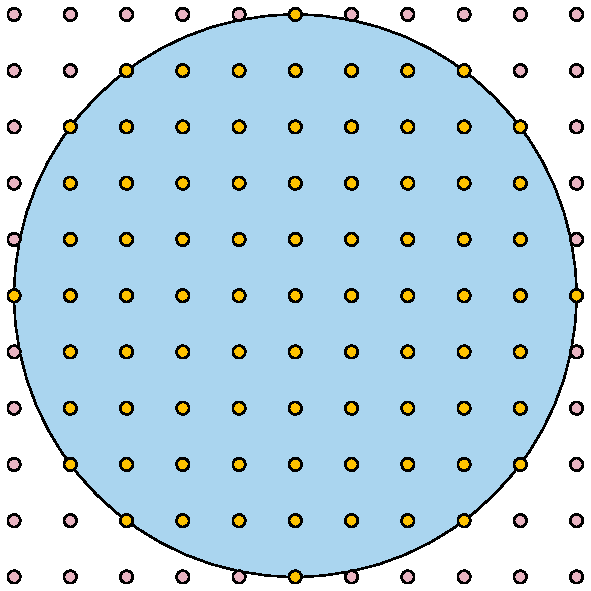
\includegraphics[width = 0.2\linewidth]{Gauss Circle Problem.pdf}
\caption{A circle with $r=5$ units bounding 81 integer points. $N(r) = 81 \sim\pi r^2\approx78.54$}
\end{figure}
% \begin{SCfigure}
% \centering
% 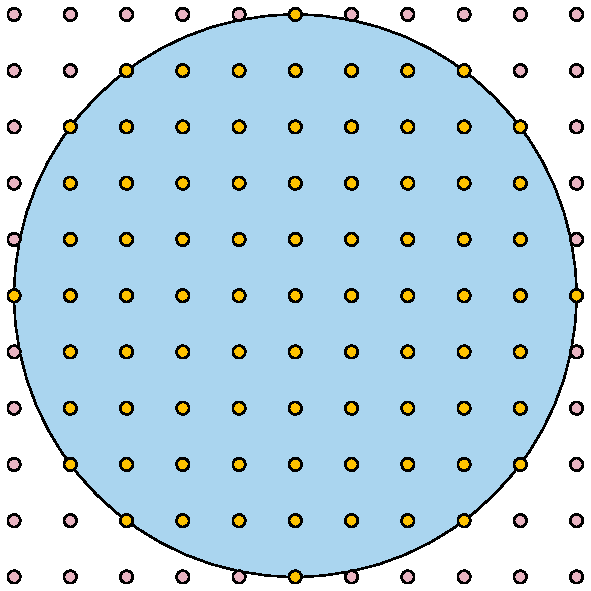
\includegraphics[width = 0.2\linewidth]{Gauss Circle Problem.pdf}
% \caption{A circle with $r=5$ units bounding 81 integer points. $N(r) = 81 \sim\pi r^2\approx78.54$}
% \end{SCfigure}
\vspace*{-1em}
Consider the subproblem of finding $M(i)$ -- the number of $(x,y) \in \mathbb{Z}^2$ such that $x^2+y^2=i$ where $i\in\{;0,1,\ldots,n\}.$ %$0\leq i\leq r^2=n$.
\\Clearly $\displaystyle N(r)=\sum_{i=0}^{r^2} M(i) \rightarrow N(\sqrt{n})=\sum_{i=0}^{n} M(i)$. Now,\vspace*{-1em}
\begin{equation}
	M(i) = 4\sum_{j|n}\chi(j)\quad\text{where}\quad\chi(n)=\begin{cases} 
      1 & \text{if $n\%4=1$}\\
      -1 & \text{if $n\%4=3$}\\
      0 & \text{else}
   \end{cases}
\end{equation}
\textbf{Problem Statement:}\\
Calculate $N(\sqrt{n})$ for a given $n$; i.e. the number of lattice points $(x,y)$ such that $x^2+y^2\leq n$.
\begin{testcasesFunction}
	{$t$ \hfill(number of test cases, an integer)\\
	$n_1\ n_2\ \ldots\ n_t$ \hfill($t$ space seperated integers for each testcase)}
	{$N(\sqrt{n_i})$ \hfill(each test case space seperated)}
	{$1 < n_i \leq 10^{7}$}
	{\texttt{int X(int n)} -- returns $\chi(n)$\\
	\texttt{int count\_lattice\_points(int n)} -- returns $M(n)$}
	{15\\0 1 2 3 5 10 20 30 50 100 1000 10000 100000 1000000 10000000}
	{1 5 9 9 21 37 69 97 161 317 3149 31417 314197 3141549 31416025}
	{https://github.com/paramrathour/CS-101/tree/main/Starter Codes/Gauss Circle Problem.cpp}
\end{testcasesFunction}
\begin{noteI}
Does the last few outputs look familiar? How can this happen? :o\\
Also, if the last output took a long time then think how you can do the calculations faster?
\end{noteI}
\begin{funvideo}
\href{https://youtu.be/NaL_Cb42WyY}{Pi hiding in prime regularities -- 3Blue1Brown}\\
\href{https://youtu.be/VftM4LpTrkI}{Your New Favorite Formula For Pi -- BriTheMathGuy}
\end{funvideo}
\documentclass[../../Problems]{subfiles}
\begin{document}
\subsection{Euler's Totient Function}\label{pp:eulertotient}
Euler's totient function $\varphi(n)$ is the number of positive integers $\leq n$ that are co-prime to $n$.\\
A simple apporach to calculating this function is to count the integers $i$'s such that $1\leq i\leq n$ and $\gcd(i,n) = 1$.\\
But there is a \emph{better} way using the Euler's Product Formula
\begin{equation}
	\varphi (n)=n\prod _{p\mid n}\left(1-{\frac {1}{p}}\right)\qquad\text{For all primes $p\leq n$}
\end{equation}
So, if  ${\displaystyle n=p_{1}^{k_{1}}p_{2}^{k_{2}}\cdots p_{r}^{k_{r}}}$, where ${\displaystyle p_{1},p_{2},\ldots ,p_{r}}$ are the distinct primes dividing $n$
% \begin{equation}
% 	{\displaystyle \varphi (n)=n(p_{1}{-}1)\,(p_{2}{-}1)\cdots (p_{r}{-}1)}
% \end{equation}
\begin{equation*}
	{\displaystyle \varphi (n)=p_{1}^{k_{1}-1}(p_{1}{-}1)\,p_{2}^{k_{2}-1}(p_{2}{-}1)\cdots p_{r}^{k_{r}-1}(p_{r}{-}1)}
\end{equation*}
\textbf{Problem Statement:}\\
Calculate $\varphi(n)$ for a given $n$

\begin{testcasesFunction}
	{$t$ \hfill(number of test cases, an integer)\\
	$n_1\ n_2\ \ldots\ n_t$ \hfill($t$ space seperated integers for each testcase)}
	{$\varphi(n_i)$ \hfill(each test case on a newline)}
	{$1 < n_i \leq 10^{9}$}
	{\texttt{int totient(int n)} -- returns $\varphi(n)$}
	{13\\1 4 8 20 44 69 97 120 2520 55440 277200 720720 88888888}
	{1\\2\\4\\8\\20\\44\\96\\32\\576\\11520\\57600\\138240\\12690687}
	{https://github.com/paramrathour/CS-101/tree/main/Starter Codes/Euler's Totient Function.cpp}
\end{testcasesFunction}
\begin{funvideo}
\href{https://youtu.be/NsjsLwYRW8o}{Prime Pyramid (with 3Blue1Brown) -- Numberphile}
\end{funvideo}
\end{document}
\subsection{Regular Star Polygon}{\label{pp:regularstarpolygon}}
A regular star polygon is a self-intersecting, equilateral equiangular polygon. It is denoted by Schl\"afli symbol $\{n/m\}$ where $n$ is the number of vertices and $m$ is the density (sum of the turn angles of all the vertices \ 360\textdegree).
\vspace{-1em}\paragraph{Construction via vertex connection} Connect every $m$\textsuperscript{th} point out of $n$ points regularly spaced on a circle.\\
For example, check out the demo videos for constructing \href{https://github.com/paramrathour/CS-101/tree/main/Media/Regular Star Polygon/7-2.mkv}{$\{7,2\}$} and \href{https://github.com/paramrathour/CS-101/tree/main/Media/Regular Star Polygon/7-3.mkv}{$\{7,3\}$}.\\
So a seven-pointed star can be obtained in two-ways,\\
By connecting vertex 1 to 3, then 3 to 5, then 5 to 7, then 7 to 2, then 2 to 4, then 4 to 6, then 6 to 1 or by\\
By connecting vertex 1 to 4, then 4 to 7, then 7 to 3, then 3 to 6, then 6 to 2, then 2 to 5, then 5 to 1.

\textbf{Problem Statement:}\\
Construct the $\{n/m\}$ regular star polygon for given $n,m$.
\begin{testcasesFunction}
	{$m\ n$ \hfill(2 space seperated integers)}
	{Regular Star Polygon with Schl\"afli symbol $\{n/m\}$}
	{$1 \leq n \leq 50$, $1 \leq m < n/2$}
	{void regular\_star\_polygon(int n, int m) -- draws the correspoding regular star polygon}
	{See \ref{fig:regularstarpolygon}.}
	{See \ref{fig:regularstarpolygon}.
	\begin{figure}[H]
	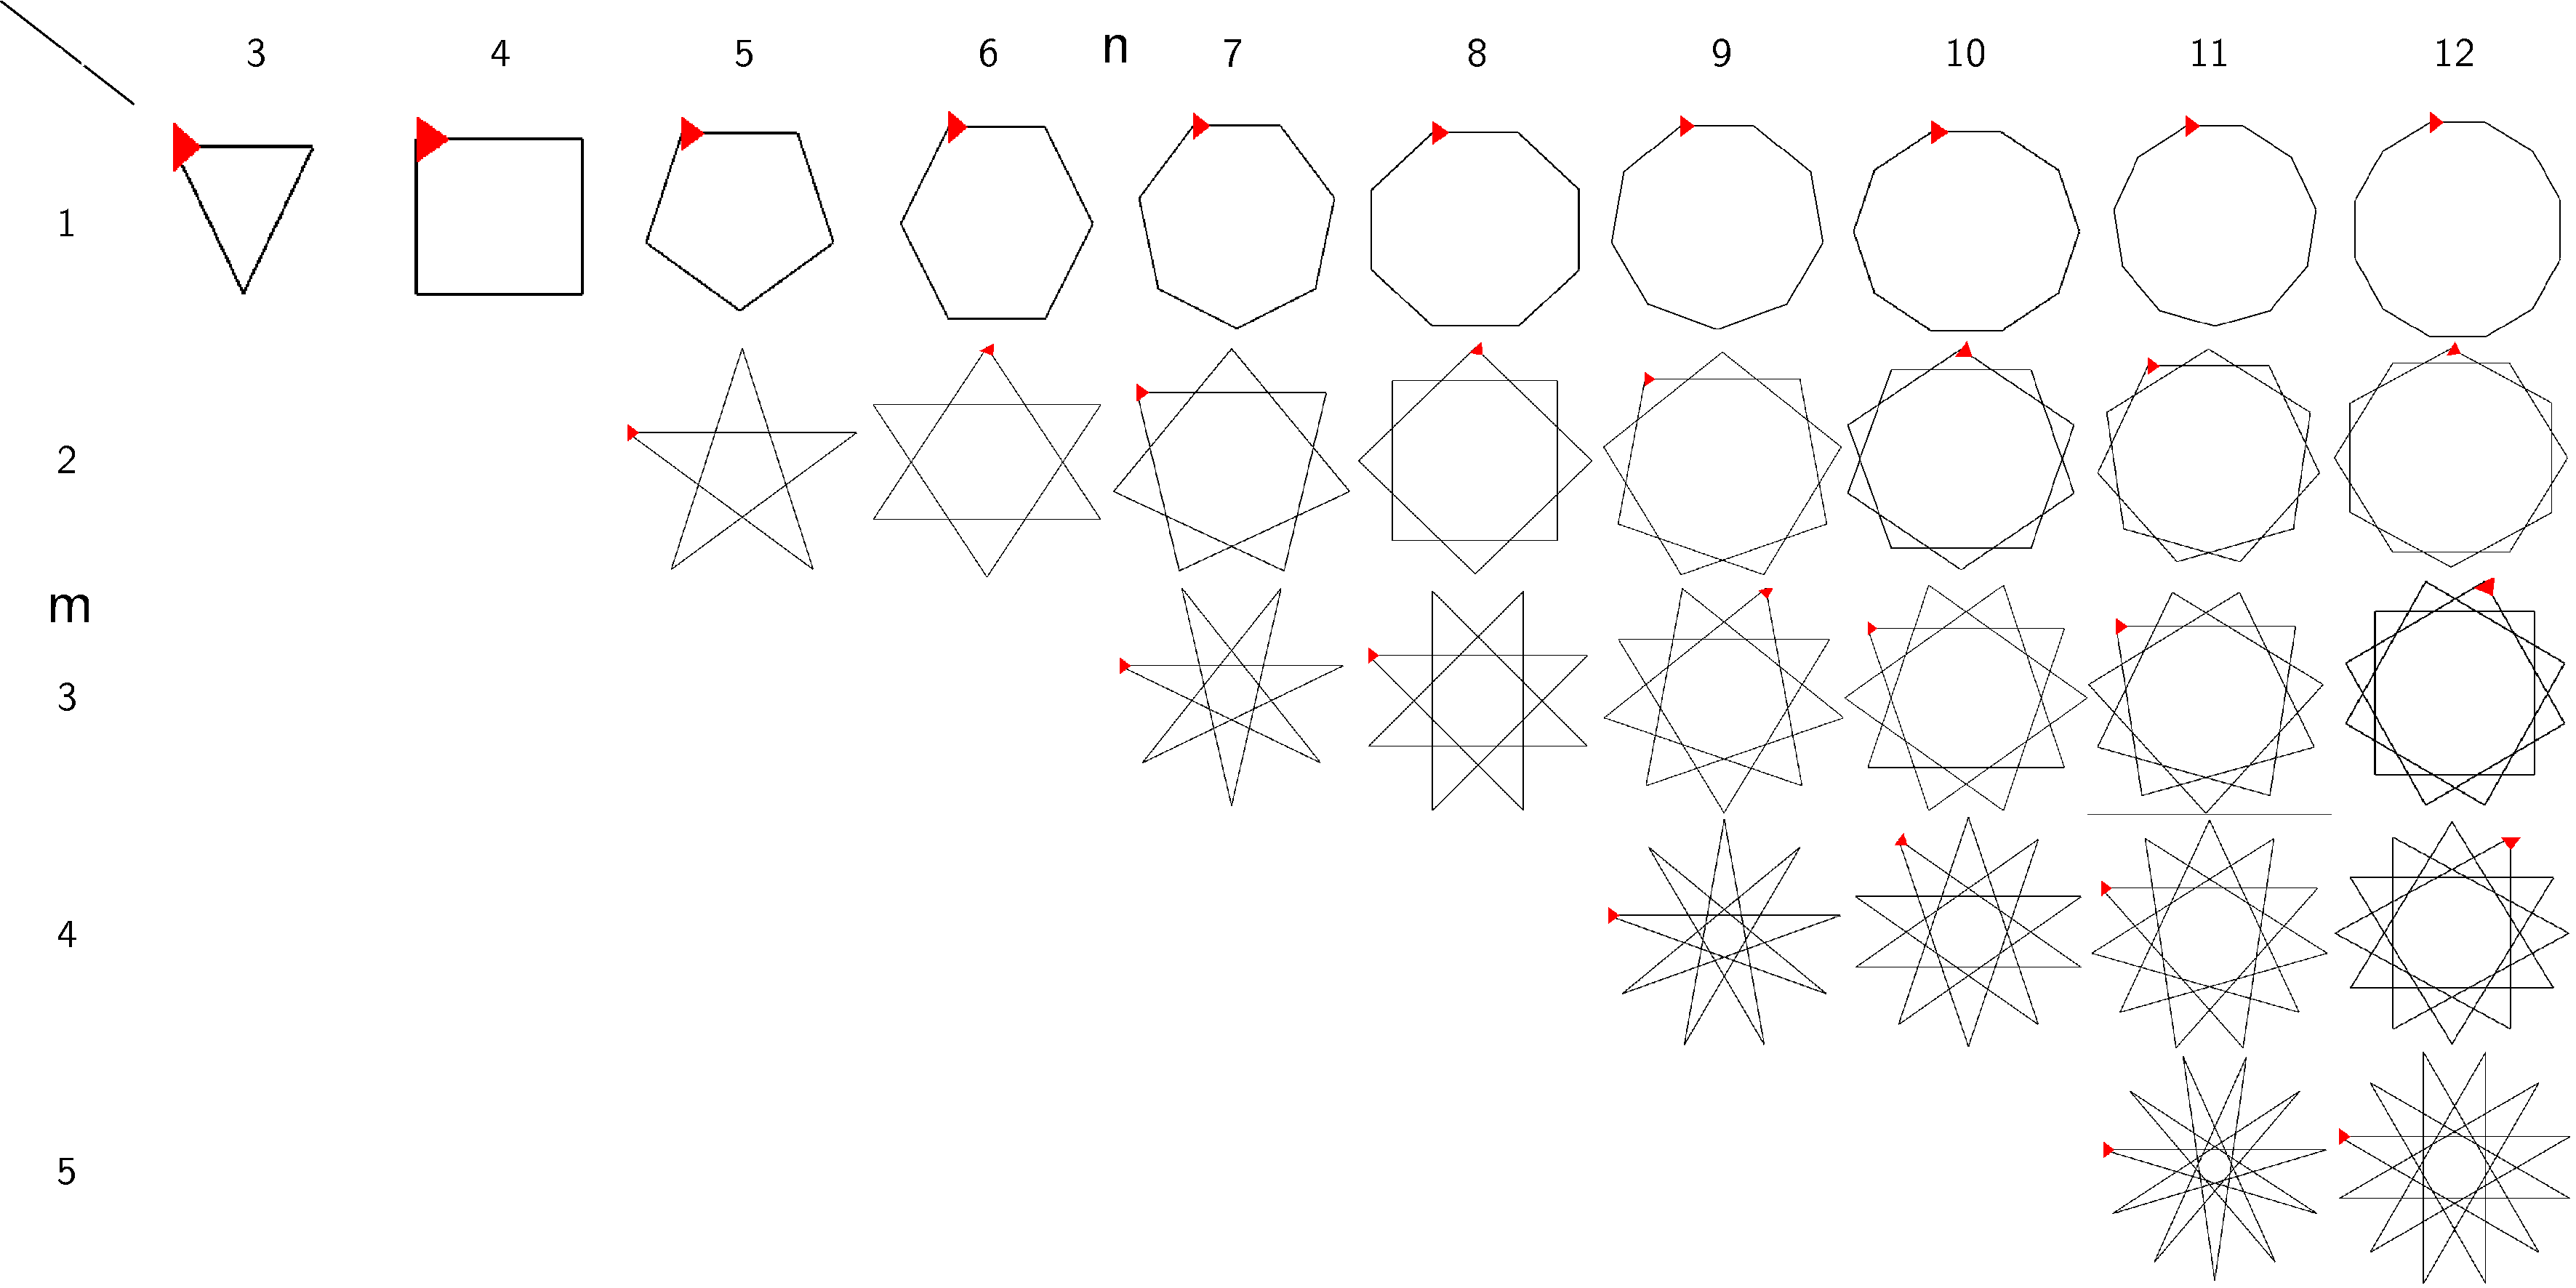
\includegraphics[width = \linewidth]{Regular Star Polygon.pdf}
	\caption{Some inputs $m,n$ and their correspoding star polygons in a tabular fashion.}
	\label{fig:regularstarpolygon}
	\end{figure}
	}
	{https://github.com/paramrathour/CS-101/tree/main/Starter Codes/Regular Star Polygon.cpp}
\end{testcasesFunction}
\begin{funvideo}
\href{https://youtu.be/oEN0o9ZGmOM}{The 3-4-7 miracle. Why is this one not super famous? -- Mathologer}
\end{funvideo}